\documentclass[conference]{IEEEtran}
\IEEEoverridecommandlockouts
% The preceding line is only needed to identify funding in the first footnote. If that is unneeded, please comment it out.
%Template version as of 6/27/2024

\usepackage{cite}
\usepackage{amsmath,amssymb,amsfonts}
\usepackage{algorithmic}
\usepackage{graphicx}
\usepackage{textcomp}
\usepackage{xcolor}
\usepackage[colorlinks=true, allcolors=blue]{hyperref}
\usepackage{subcaption}
\pagestyle{plain}

\def\BibTeX{{\rm B\kern-.05em{\sc i\kern-.025em b}\kern-.08em
    T\kern-.1667em\lower.7ex\hbox{E}\kern-.125emX}}
\begin{document}

\title{An NDN-Based DNS Protocol for Improved Security and Efficiency in Edge Devices*\\
{\footnotesize \textsuperscript{*}Note: Sub-titles are not captured for https://ieeexplore.ieee.org and
should not be used}
\thanks{Identify applicable funding agency here. If none, delete this.}
}

\author{\IEEEauthorblockN{1\textsuperscript{st} Sameer G Kulkarni}
\IEEEauthorblockA{\textit{Computer Science and Engineering (Asst. Prof.)} \\
\textit{Indian Institute of Technology Gandhinagar}\\
Gandhinagar, India \\
sameergk@iitgn.ac.in}
\and
\IEEEauthorblockN{2\textsuperscript{nd} Mithil Pechimuthu}
\IEEEauthorblockA{\textit{Computer Science and Engineering (Student)} \\
\textit{Indian Institute of Technology Gandhinagar}\\
Gandhinagar, India \\
pechimuthumithil@iitgn.ac.in}
\and
\IEEEauthorblockN{3\textsuperscript{rd} Sachin Jalan}
\IEEEauthorblockA{\textit{Computer Science and Engineering (Student)} \\
\textit{Indian Institute of Technology Gandhinagar}\\
Gandhinagar, India \\
jalansachin@iitgn.ac.in}
\and
\IEEEauthorblockN{4\textsuperscript{th} Tirth Patel}
\IEEEauthorblockA{\textit{Computer Science and Engineering (Student)} \\
\textit{Indian Institute of Technology Gandhinagar}\\
Gandhinagar, India \\
pateltirth@iitgn.ac.in}
% \and
% \IEEEauthorblockN{5\textsuperscript{th} Given Name Surname}
% \IEEEauthorblockA{\textit{dept. name of organization (of Aff.)} \\
% \textit{name of organization (of Aff.)}\\
% City, Country \\
% email address or ORCID}
% \and
% \IEEEauthorblockN{6\textsuperscript{th} Given Name Surname}
% \IEEEauthorblockA{\textit{dept. name of organization (of Aff.)} \\
% \textit{name of organization (of Aff.)}\\
% City, Country \\
% email address or ORCID}
}

\maketitle

\begin{abstract}
The Domain Name System (DNS) protocol has remained unchanged since its inception in 1983. While it is efficient for general computing, the increasing importance and number of edge devices and IoT may reveal that the current DNS protocol implementation can be power-hungry, slow and insecure. Experiments showed that the DNS protocol and its implementation have inefficiencies that cause overheads in resource-constrained environments, such as IoT devices with limited energy budgets. We motivate the need for a new DNS protocol and state the aspects that can be improved upon. The details of the experiments conducted are also present in this document. Finally, we propose a new DNS protocol based on Named Data Networking (NDN) that addresses security and efficiency issues while having a low power footprint. We used the ICARUS-ICN simulator to verify these claims; the results are presented in this document.
\end{abstract}

\begin{IEEEkeywords}
DNS, NDN, Security, Efficiency, Edge Devices, IoT
\end{IEEEkeywords}

\section{Introduction}
\subsection{Background on DNS}
The Domain Name System (DNS) is a hierarchical and decentralized naming system that serves as the backbone of modern Internet communication. It translates human-readable domain names, such as \texttt{www.example.com}, into machine-readable numerical IP addresses, enabling devices to locate and communicate with one another over the Internet. This process is crucial for the functionality of websites, email services, and numerous other online applications \cite{mockapetris1983dns}.

DNS was introduced in 1983 to address the challenges posed by maintaining a centralized host file for mapping domain names to IP addresses. Despite its robustness and scalability, the DNS protocol has largely remained unchanged since its inception. This legacy design leaves DNS vulnerable to various security threats, such as cache poisoning, spoofing, and distributed denial-of-service (DDoS) attacks. For example, let's say we want to resolve the domain name like "iitgn.ac.in," into IP addresses like 72.1.241.188, that machines use to address each other. Usually, all of the DNS operates using a recursive query mechanism, where a DNS resolver iteratively queries multiple DNS servers to resolve a domain name, starting from the root servers (contain info about .com, in, etc...) through the top-level domain (TLD) servers (provide .com, .in,  etc...), and down to the authoritative servers. Figure \ref{fig:dns-overview} shows the exact steps taken to resolve our example domain "iitgn.ac.in". 

\begin{figure}[htbp]
    \centering
    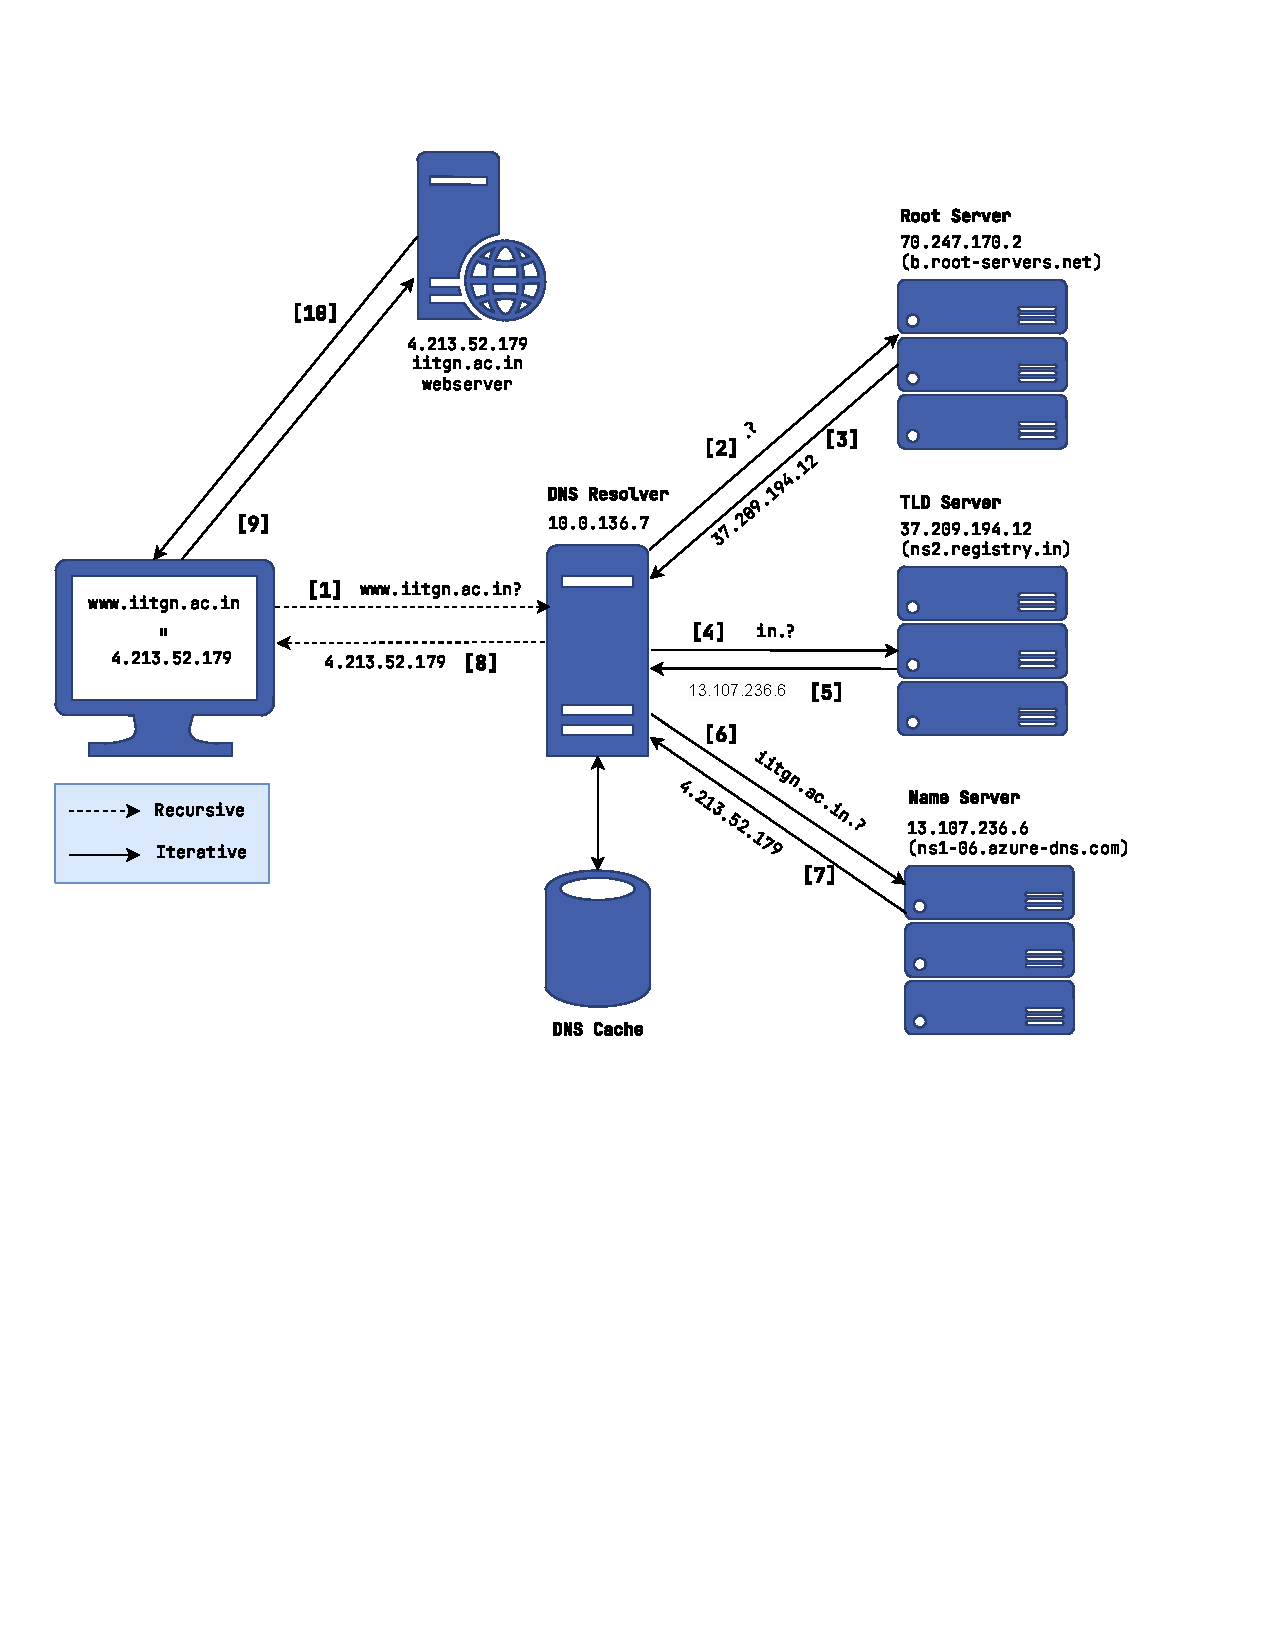
\includegraphics[width=1\linewidth,trim={0 10cm 0 2cm},clip]{images/dns-overview.pdf}
    \caption{DNS Architecture}
    \label{fig:dns-overview}
\end{figure}

\subsection{Integrating Security: DNS-SEC}
To mitigate these vulnerabilities, DNS Security Extensions (DNS-SEC) were introduced to enhance the protocol with mechanisms like digital signatures for DNS records. Figure \ref{fig:DNS-SEC-overview} represents the steps involved in DNS-SEC. 

\begin{figure}[htbp]
    \centering
    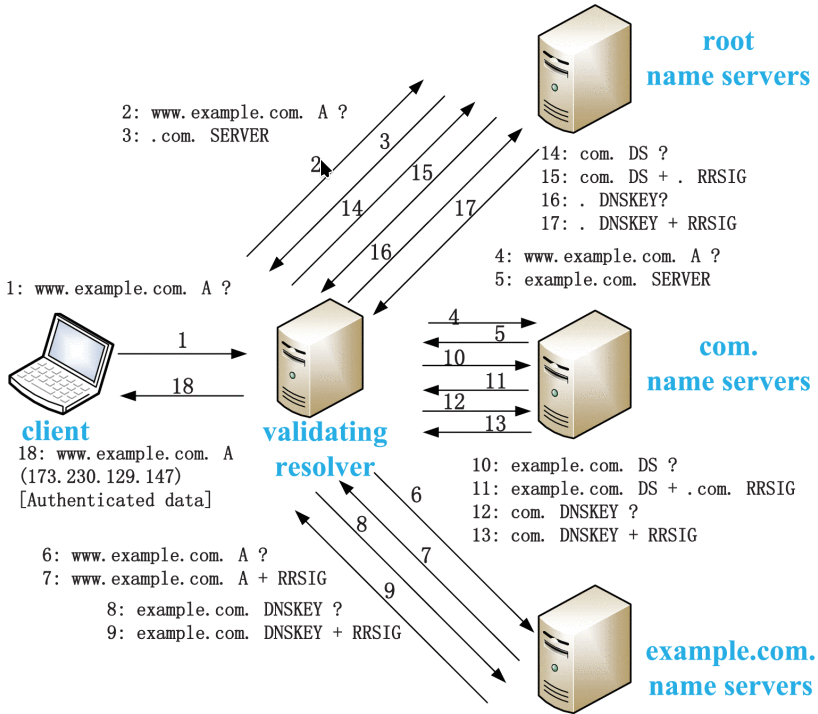
\includegraphics[width=0.9\linewidth]{images/dnssec-overview.png}
    \caption{DNS-SEC Architecture \cite{8653281}}
    \label{fig:DNS-SEC-overview}
\end{figure}

On comparing figures \ref{fig:dns-overview} and \ref{fig:DNS-SEC-overview} we can see that while DNS-SEC improves the security of DNS, it is complex and has hight computational overhead \cite{8653281}. In addition to this overhead, implementation of DNS-SEC requires huge time and human resouces and lack of global consesus \cite{polo-2022} prevent widespread adoption of DNS-SEC. This overhead is particularly problematic for resource-constrained devices, such as those used in IoT environments, which may lack the processing power or battery capacity to handle the added burden. The cryptographic operations involved in DNS-SEC, such as signature verification, are resource-intensive and can quickly deplete the limited battery life of edge devices. Figures \ref{fig:dns-cycles} and \ref{fig:dns-energy} show the resource consumed for plain DNS resolution. This only increases when complex protocols such as DNS-SEC is used. Additionally, the added latency from DNS-SEC validation may impact time-sensitive applications, such as real-time monitoring and control systems. Furthermore, frequent DNS lookups increase network overhead, which is particularly burdensome for low-power wide-area networks (LPWANs) that are commonly used in IoT deployments. These inefficiencies underline the need for alternative approaches or optimizations to make DNS suitable for edge environments. The section \ref{Measuring Protocol Inefficiencies} explains how we examines the DNS protocol and encountered some pain points.

% \subsection{Impact on Edge Devices}
% \label{Impact on Edge Devices}
% Edge devices, including IoT devices, face significant challenges when using DNS due to their constrained resources. DNS queries can introduce latency and require computational resources to process responses, particularly when DNS-SEC is employed. The cryptographic operations involved in DNS-SEC, such as signature verification, are resource-intensive and can quickly deplete the limited battery life of edge devices. Figures \ref{fig:dns-cycles} and \ref{fig:dns-energy} show the resource consumed for plain DNS resolution. This only increases when complex protocols such as DNS-SEC is used. Additionally, the added latency from DNS-SEC validation may impact time-sensitive applications, such as real-time monitoring and control systems.

% Furthermore, frequent DNS lookups increase network overhead, which is particularly burdensome for low-power wide-area networks (LPWANs) that are commonly used in IoT deployments. These inefficiencies underline the need for alternative approaches or optimizations to make DNS suitable for edge environments.

\begin{figure}[htbp]
    \centering
    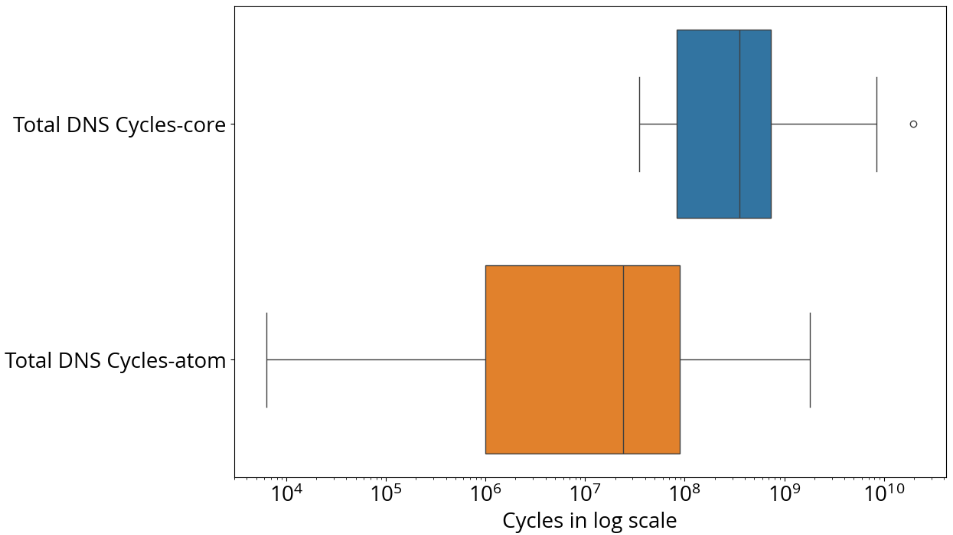
\includegraphics[width=0.9\linewidth]{images/cycles.png}
    \caption{This box plot shows the cycles (in log scale) consumed in the DNS resolution of every domain required to load a page, for the 1000 website we tested.}
    \label{fig:dns-cycles}
\end{figure}
\begin{figure}[htbp]
    \centering
    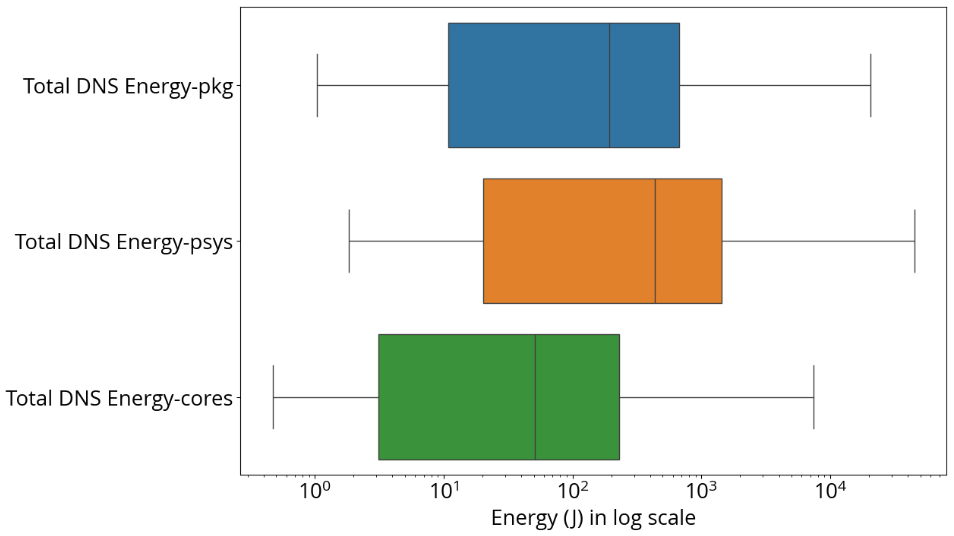
\includegraphics[width=0.9\linewidth]{images/energy.png}
    \caption{This box plot shows the energy (J) (in log scale) consumed in the DNS resolution of every domain required to load a page, for the 1000 website we tested.}
    \label{fig:dns-energy}
\end{figure}

\section{Measuring Protocol Inefficiencies}
\label{Measuring Protocol Inefficiencies}
The DNS protocol and it's implementation exhibits several inefficiencies. We performed several experiments which led us to thhe conclusion that the DNS protocol must be tweaked based on pattern observed in the requests for domain name resolution. We collected the list of the top 1000 domains from cloudflare \cite{cloudflare}. We then explored several tools but weren't satisfied with the depth of analysis that they allowed for. Hence, we chose to build and develop or own scripts to analyse the DNS protocol. 

\subsection{Capturing Packets}
After getting the top 1000 domains, we built a sandboxed environment using Docker containers to simulate the page load of these top 1000 domains and capture the packets. This was necessary as we didn't want any other network traffic flowing throught the same interface interfere with our experiments. We also kept a time out of 10 seconds to prevent being stuck on domains unaccessible throught NKN network. Furthermore, we took extra care to make sure that the DNS data we recieved was not cached and queries took the comple route through the resolvers. After going through the GNU manual for wget \cite{wget}, we concluded that running the following command in a docker container will do the trick. wget --no-dns-cache --no-verbose --timeout 10 -t 1 -c -E -H -k -K -p domain

\subsection{Analyzing the Captured Packets}
We developed several python scripts to analyse the captired packets. These scripts can be found in our \href{https://github.com/SachinJalan/DNS-Renaissance}{Github repository}. By leveraging tools like perf and dig (with special care not to use cached records) we collected the following information from the captured packets:
\begin{itemize}
    \item \textbf{Total Packets}: The total number of packets captured.
    \item \textbf{Total Bytes}: The total bytes of data exchanged.
    \item \textbf{Total DNS Packets}: The total number of DNS-specific packets.
    \item \textbf{Total DNS Bytes}: The total bytes of DNS-related traffic.
    \item \textbf{Total Time}: The total duration for complete page load.
    \item \textbf{Total DNS Time}: The total duration for DNS resolution.
    \item \textbf{Time to First Byte (TTFB)}: The time taken to receive the first byte of the response.
    \item \textbf{Total DNS Cycles}: The number of CPU cycles used during DNS resolution using the \texttt{perf} tool.
    \item \textbf{Total DNS Energy}: The energy consumption during DNS resolution, captured using the \texttt{perf} tool.
    \item \textbf{Visited Domains}: A list of all the domains involved in the page load with there respective record types.
\end{itemize}
These captured parameters were then analsed and plotted.

\subsection{Analysis and Plots}
We first analysed the packets that were involved in loading the complete page. We noticed that for the resolution of a single domain, various other domains were also queried for. For example, loading iitgn.ac.in required loading fonts.googleapis.com, googletagemanager, cdn.usefathom.com, www.facebook.com. and many more other thant iitgn.ac.in. Figure \ref{fig:n_visited-domains} shows that a significant number of websites requied multiple domain namees to be resolved. Furthermore, we also noticed that a single domain was repeatedly queried for multiple times throught the average pade load packet capture.

\begin{figure}[htbp]
    \centering
    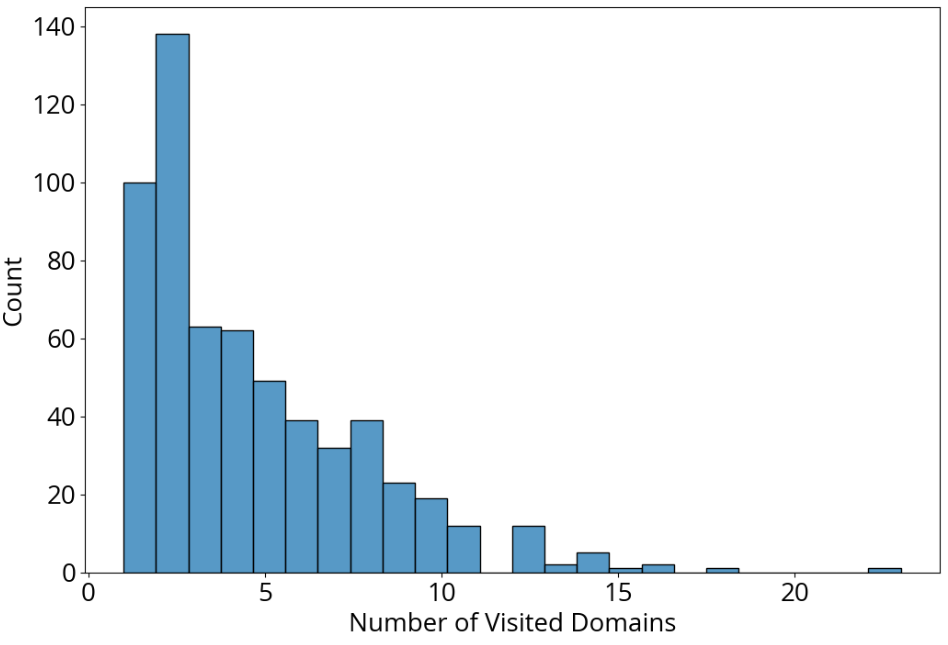
\includegraphics[width=0.9\linewidth]{images/n_visited-domains.png}
    \caption{This histogram shows the count of websites (out of 1000) vs the of number of distinct domains visited.}
    \label{fig:n_visited-domains}
\end{figure}

Another heuristic we observed was that when an A record was queried, an AAAA query also accompanied in most cases. Figure \ref{fig:qtypes} shows this. 

\begin{figure}[htbp]
    \centering
    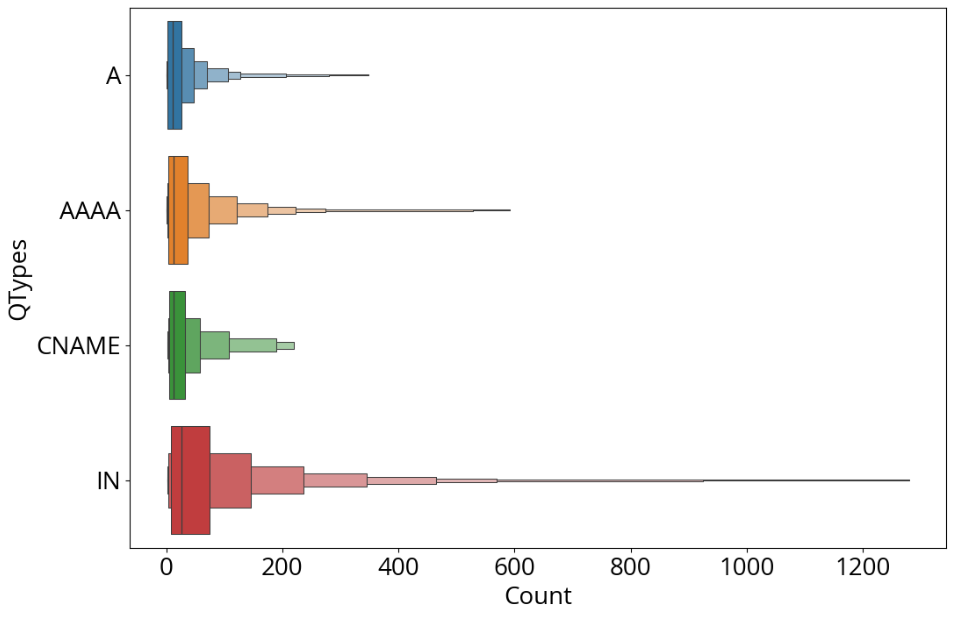
\includegraphics[width=0.9\linewidth]{images/qtypes.png}
    \caption{This boxen plot shows counts of the qtypes encountered in the page load of the top 1000 websites. Note how only A, AAAA and CNAME were the record types that were requested for.}
    \label{fig:qtypes}
\end{figure}

Further more we noticed that in one DNS query packet, only a single question was sent. However, the protocol allowed for multiple questions. This and and the above mentioned observations caused the DNS resolution to take a significant amount of time, packets and bytes of the total page load. Figures \ref{fig:bytes-time-packets} shows this overhead caused by the current deployment of the DNS protocol. Figures \ref{fig:time-ratio}, \ref{fig:packet-ratio} and \ref{fig:bytes-ratio} are also provided for reference.

\begin{figure}[htbp]
    \centering
    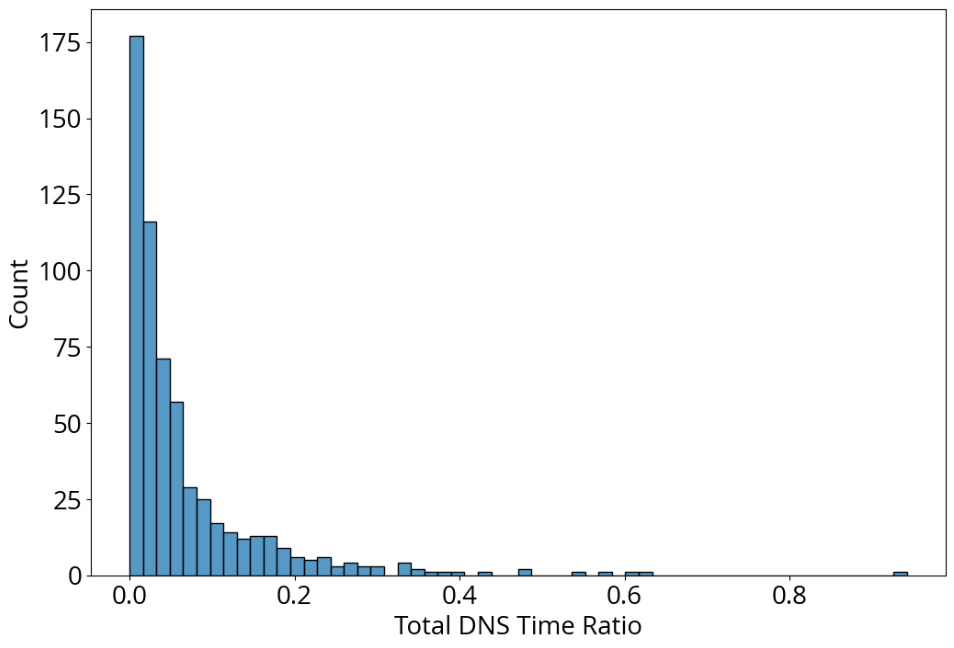
\includegraphics[width=0.9\linewidth]{images/time-ratio.png}
    \caption{This box plot shows the counts of the domains vs the ratio of time spent in DNS resolution to total page load time.}
    \label{fig:time-ratio}
\end{figure}

\begin{figure}[htbp]
    \centering
    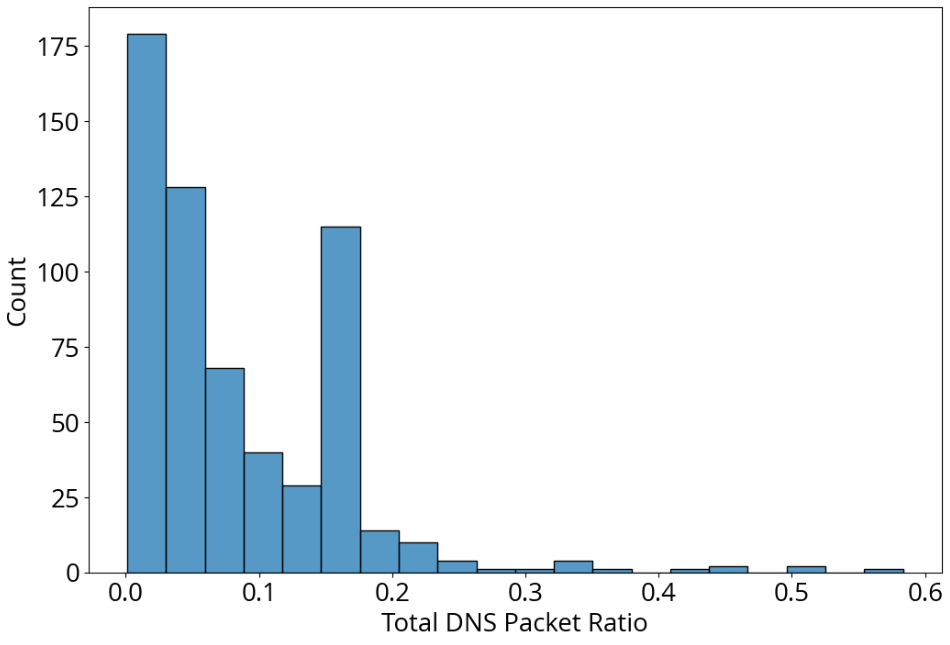
\includegraphics[width=0.9\linewidth]{images/packet-ratio.png}
    \caption{This box plot shows the counts of the domains vs the ratio of packets spent in DNS resolution to total packets for loading the complete page.}
    \label{fig:packet-ratio}
\end{figure}

\begin{figure}[htbp]
    \centering
    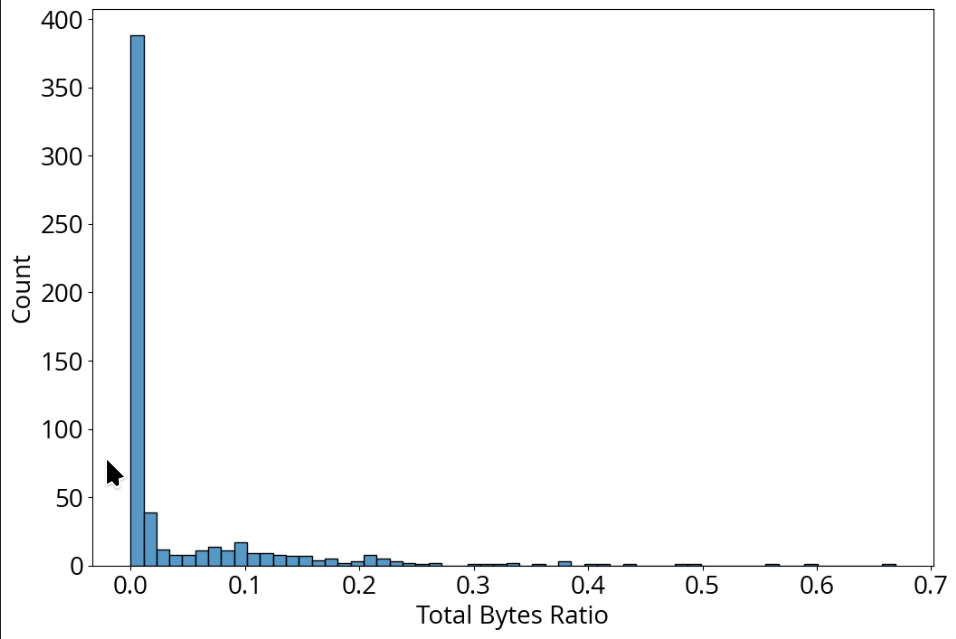
\includegraphics[width=0.9\linewidth]{images/bytes-ratio.png}
    \caption{This box plot shows the counts of the domains vs the ratio of bytes spent in DNS resolution to total bytes through the network to load the page.}
    \label{fig:bytes-ratio}
\end{figure}

\begin{figure}[htbp]
    \centering
    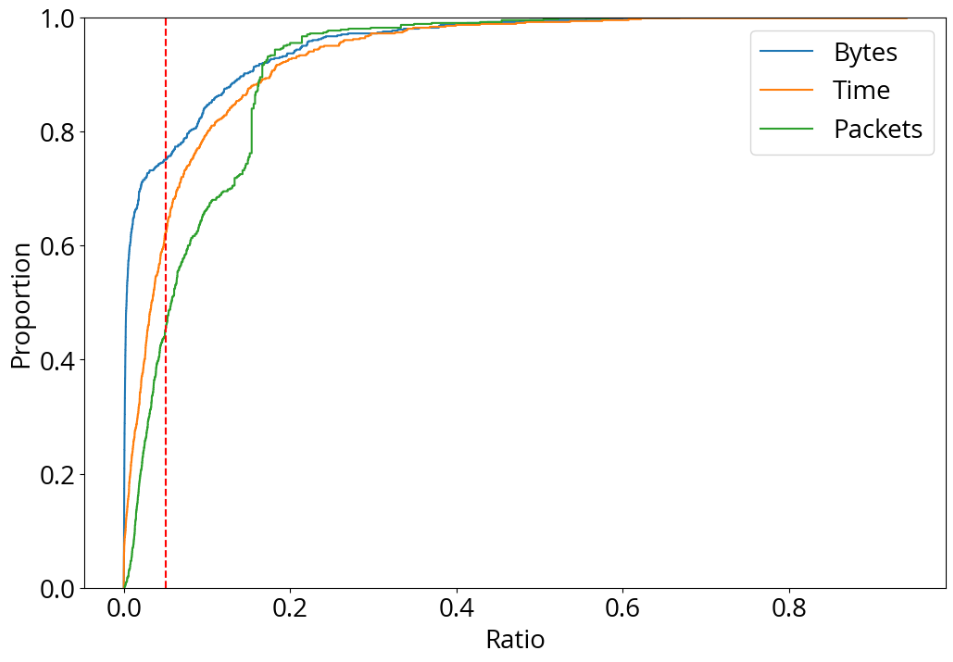
\includegraphics[width=0.9\linewidth]{images/bytes-time-packets.png}
    \caption{This is the CDF of the ratio of byte, time taken, and packets involved in DNS resolution. The 5\% critical region is also marked through a dashed red vertical line. From this, we infer
    that 60\%, 40\%, and 35\% of websites are beyond the
    5\% limit for bytes, time and packets taken respectively.}
    \label{fig:bytes-time-packets}
\end{figure}

We also observerd that almost 7 bytes corresponding to the aa, z qdcount, nscount, arcount fields in the DNS header were never used in the page load of the top 1000 websites. We also noted that shift of transport layer protocol from UDP to TCP were very rare. It occured 0.3\% out of the total 17277 DNS queries. These were mostly for AAAA records. This tells us that the DNS packets are small enough to fit into one UDP dataframe. Switching to TCP is rare, but when it occurs, we see about 1.2x increase in DNS resolution times.

Furthermore we also checked if using a delegation like resolution other than the supported recursive and iterative would work in reducing the DNS resolution times. Delegation mode is where the name server is delegated the responsibility to respond back to the client with the record the client requested for. Since delegated mode is not supported natively by DNS, we measured it by calculating the time for resolving recursively ($RTT_r$), and the ping time to the name server ($RTT_p$) and finally calculating the delegation time ($RTT_d$) as $RTT_d = \frac{1}{2}RTT_r + \frac{1}{2}RTT_p$. However delegated mode though theoretically involved less DNS packets, didn't provide much benefit as seen in figure \ref{fig:delegation} where only 5\% of the DNS requests encountered benefited from delegating the name server to return the answer to the client.

\begin{figure}[htbp]
    \centering
    \begin{subfigure}[b]{0.9\linewidth}
        \centering
        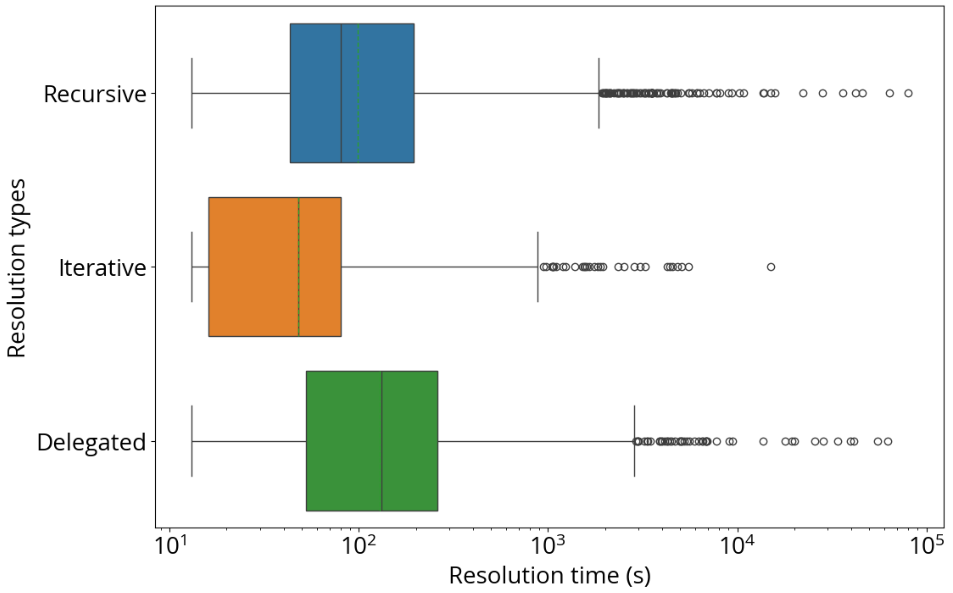
\includegraphics[width=\linewidth]{images/delegation-box.png}
        \caption{}
    \end{subfigure}
    \begin{subfigure}[b]{0.9\linewidth}
        \centering
        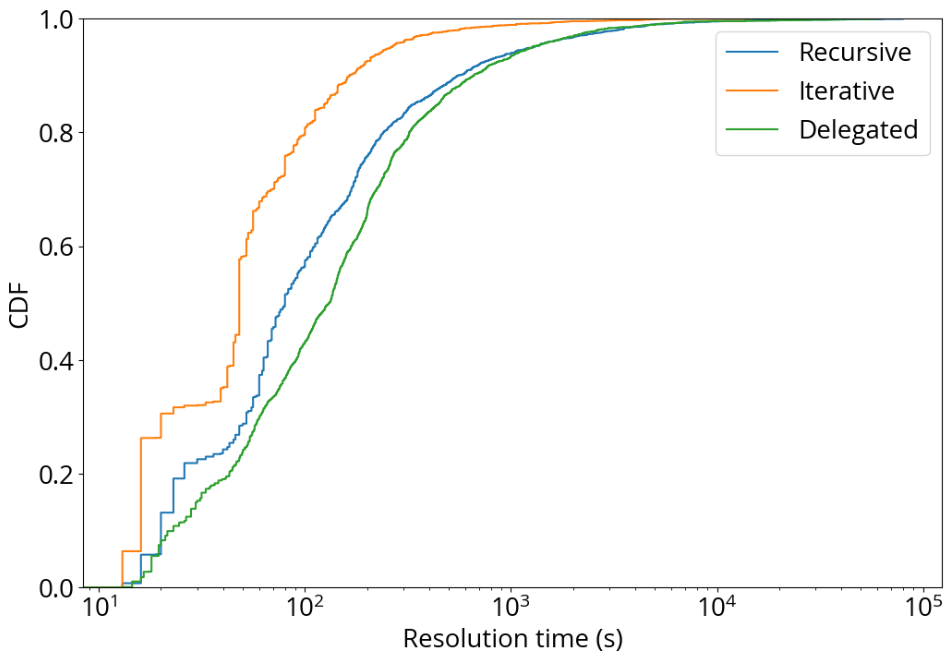
\includegraphics[width=\linewidth]{images/delegation-cdf.png}
        \caption{}
    \end{subfigure}
    \caption{The box plots (a) and the cdf plots (b) show a comparison between the resolution time taken while using recursive, iterated or delegated modes respectively.}
    \label{fig:delegation}
\end{figure}

With all this analysis, we had enough context sett to proceed further to design a new DNS protocol that will address all these ineffeciencies.

\section{Adressing the Problems: NDN-DNS}
We provide a solution that integrates the principles of Named Data Networking (NDN) to establish the foundations of a novel protocol for DNS resolution.
\subsection{Introduction to NDN}
NDN is a paradigm shift in networking, where communication is centered around named content rather than IP addresses. Instead of retrieving data from a specific location, NDN retrieves data by name, allowing efficient in-network caching and secure delivery of content.

\subsection{NDN-DNS protocol overview}

\subsection{Analysis of Proposed Solution}

\section{Related Works}

\section{Conclusion}

\bibliographystyle{plain}
\bibliography{references}
\end{document}
